\documentclass{article}%
\usepackage[T1]{fontenc}%
\usepackage[utf8]{inputenc}%
\usepackage{lmodern}%
\usepackage{textcomp}%
\usepackage{lastpage}%
\usepackage[head=40pt,margin=0.5in,bottom=0.6in]{geometry}%
\usepackage{graphicx}%
%
\title{\textbf{Gobierno levanta medidas que impedían el traslado de reses}}%
\author{CARLOS SEIJAS MENESES | @carlosgmeneses | ELEONORA DELGADO | eldelgado@el{-}nacional.com}%
\date{22/11/2018}%
%
\begin{document}%
\normalsize%
\maketitle%
\textbf{URL: }%
http://www.el{-}nacional.com/noticias/economia/gobierno{-}levanta{-}medidas{-}que{-}impedian{-}traslado{-}reses\_260683\newline%
%
\textbf{Periodico: }%
EN, %
ID: %
260683, %
Seccion: %
Economía\newline%
%
\textbf{Palabras Claves: }%
Economía\newline%
%
\textbf{Derecho: }%
2.10, %
Otros Derechos: %
, %
Sub Derechos: %
2.10.1\newline%
%
\textbf{EP: }%
NO\newline%
\newline%
%
\textbf{\textit{Gerardo Ávila, presidente de Fegalago, afirmó que en Zulia se mantiene la restricción de movilización de ganado a otras entidades. En Apure tampoco se ha acatado la orden}}%
\newline%
\newline%
%
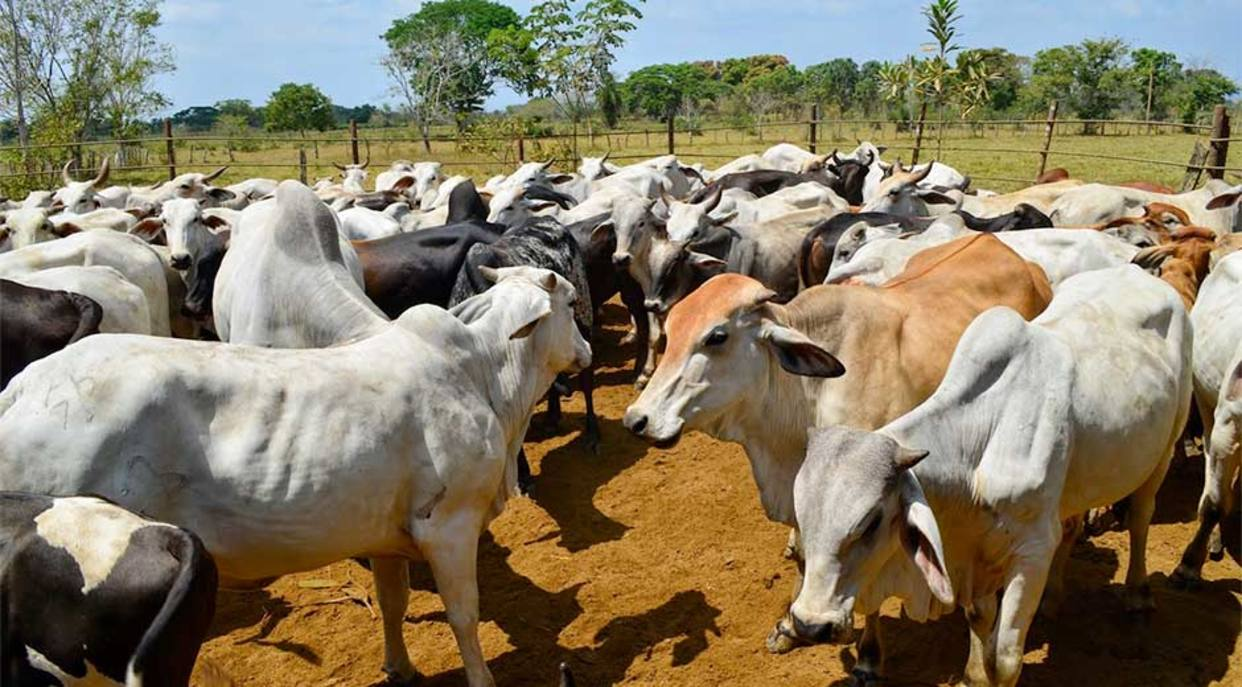
\includegraphics[width=300px]{216.jpg}%
\newline%
%
Después de que la escasez de carne alcanzó la alarmante cifra de 90\% desde que gobernadores intervinieron, hace tres meses, la cadena cárnica y fijaron precios por debajo de los costos de producción, el gobierno levantó las medidas que impedían el traslado de reses.%
\newline%
%
El artículo 1 de la resolución publicada en~la~Gaceta Oficial~41526, del 16 de noviembre, prohíbe en todo el territorio “la emisión o ejecución de cualquier restricción o gravamen que impidan el acopio, transporte, distribución, comercialización o libre movilización de alimentos”.%
\newline%
%
La orden, firmada por el Comando para el Abastecimiento Soberano y los ministerios de Industrias y Producción, de Agricultura Productiva y Tierras, de Alimentación, de Pesca y Acuicultura, y de Comercio Nacional, también prohíbe a las autoridades estadales o municipales fijar precios a los bienes.%
\newline%
%
Los gobernadores José Vásquez, de Guárico; Ramón Carrizález, de Apure; Argenis Chávez, de Barinas; Julio León Heredia, de Yaracuy; Rafael Calles, de Portuguesa, y Margaud Godoy, de Cojedes, exigían 45 bolívares por el el kilo de vaca en pie y 50 bolívares el kilo de toro en pie, hasta 60\% del rebaño que es arrimado a los mataderos.%
\newline%
%
“El gobierno se dio cuenta de que estaba atropellando al sector. En Barinas se restringía la salida del ganado a grandes centros de beneficio y de consumo como Aragua, Carabobo, Lara, Distrito Capital y Miranda, lo que generó bastante retraso y trabas. Nadie quería trabajar a pérdida”, expresó José Labrador, presidente de~la Asociación~de Productores Rurales de Barinas.%
\newline%
%
Dijo que el director regional del Instituto Nacional de Salud Agrícola Integral informó el martes que ya no había limitantes para la salida de los animales de Barinas a cualquier parte del país. Sin embargo, en los estados fronterizos hay una restricción de guiado, previa a la que ejecutaban los gobernadores de las entidades llaneras, añadió.%
\newline%
%
Gerardo Ávila, presidente de~la Federación~de Ganaderos de~la Cuenca~del Lago, afirmó que~la Gobernación~de Zulia persiste en imponer gravámenes y porcentajes sobre el ganado que se arrima a los mataderos. “Hasta este momento desconoce la orden que prohíbe tales imposiciones”, declaró.%
\newline%
%
Apure también mantiene las restricciones de movilización de ganado a otras entidades para su beneficio y comercialización, aun cuando el gobierno ordenó levantar esas medidas. Desde enero pasado, gobernaciones de estados productores de ganado y leche comenzaron a limitar el traslado de los rebaños.%
\newline%
%
En septiembre, jefes militares reunidos con productores del centro del país anunciaron el inicio de un plan piloto que consistiría en la intervención del gobierno de Nicolás Maduro en la movilización y beneficio de reses, para la posterior distribución y comercialización de la carne.%
\newline%
%
Chara Melgarejo, presidente de~la Asociación~de Ganaderos de Apure, señaló que en esa entidad los funcionarios no han acatado la resolución por lo que harán gestiones ante~la Fiscalía Superior~de Apure para que se cumpla. En el estado, las medidas restrictivas han sido de palabra y no hay documentos que las avalen. Sin embargo, las guías de movilización de ganado que son emitidas por el Instituto Nacional de Salud Agrícola Integral, son negadas.%
\newline%
%
“Aquí hay represado por lo menos 2.000 animales que tienen que ir a los mataderos del centro del país y no los hemos podido sacar porque los funcionarios del Insai se niegan, debido a que no tienen la instrucción expresa del director regional. No nos han dado las guías de movilización”, indicó Melgarejo.%
\newline%
%
El artículo 6 de la resolución establece que el incumplimiento será considerado una trasgresión a la seguridad y soberanía agroalimentaria y estará sujeto a la aplicación de la sanción de prisión de~12 a~15 años, correspondiente al delito de boicot; y de~3 a~6 años, por el delito de condicionamiento.%
\newline%
%
En Táchira las tierras son utilizadas para la ceba y cría de rebaños procedentes de Barinas y Apure. Cuando se impuso la restricción de movilización no hubo ganado para tal fin, tampoco para llevarlo a sacrificio en los mataderos industriales de la entidad que tienen capacidad para el beneficio diario de~500 a~600 reses.%
\newline%
%
Leonardo Figueroa, presidente de~la Asociación~de Ganaderos del Táchira, calificó la situación de violación al derecho de alimentación de los tachirenses.%
\newline%
%
\end{document}